\section{The Ralph Experiment: Convergent Evolution Without Specification}

The Wallfacer experiment demonstrates bottleneck migration and role fission within a single pipeline. A natural follow-up question is whether multiple independent instances, started from identical initial conditions, exhibit convergent or divergent evolutionary trajectories. To investigate this, we conducted a second experiment using a simpler pipeline that lacks Wallfacer's role differentiation.

\subsection{Setup}

We used \emph{ralph}, an autonomous agent pipeline that runs a three-phase loop: a \textbf{Thinker} analyzes the current project state and proposes exactly one goal for the next round; a \textbf{Worker} implements that goal; and a \textbf{Committer} stages all changes and pushes a commit. Unlike Wallfacer's multi-role architecture, ralph's loop is fixed: no Cartographer, no Critic, no fission. The pipeline persists execution history as JSON logs, enabling the Thinker to condition each new goal on the full trajectory of prior rounds.

We pointed ralph at three empty Git repositories with no seed task, no prompt, and no specification of what to build. The only input was an empty directory. Each instance used the same LLM substrate (Claude) and the same pipeline configuration. We let all three run autonomously; two completed 42 rounds and one completed 33 rounds before being stopped. Table~\ref{tab:ralph_repos} summarizes the resulting codebases.

\begin{table}[t]
\small
\caption{Three codebases generated by ralph from empty repositories with no seed task. All three independently converged on cellular automaton simulators.}
\label{tab:ralph_repos}
\begin{tabular}{@{}llrrr@{}}
\toprule
\textbf{Repository} & \textbf{Lang.} & \textbf{LOC} & \textbf{Funcs} & \textbf{Cost} \\
\midrule
Explorer   & C      & 10{,}876 & 133 & \$89.66 \\
Sandbox    & Python & 14{,}727 & 509 & \$56.87 \\
Simulator  & Python & 12{,}336 & 285 & \$57.80 \\
\bottomrule
\end{tabular}
\end{table}

\subsection{Observations}

\begin{figure}[t]
\centering
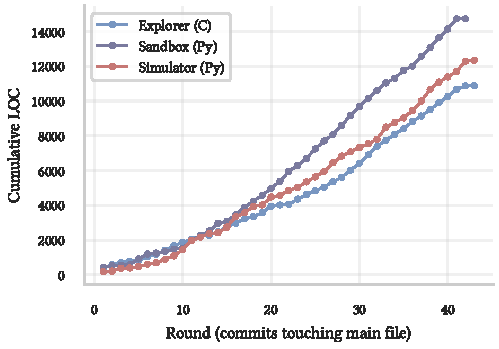
\includegraphics[width=\columnwidth]{figures/ralph_loc_growth.pdf}
\caption{Cumulative lines of code across three independently initialized repositories. All three converged on cellular automaton implementations despite receiving no seed task. Growth is monotonically increasing with near-zero churn (3.9\%, 0.5\%, and 3.0\% deletion ratios respectively).}
\label{fig:ralph_loc}
\end{figure}

\textbf{Observation 4: Convergent goal selection from null initial conditions.} All three instances independently chose to build a cellular automaton simulator as their first goal and continued developing it for every subsequent round. This convergence occurred without any seed task, prompt engineering, or inter-instance communication. The ``null'' initial condition is, of course, not truly null: it includes the LLM's entire training distribution, which implicitly encodes priors over what constitutes an interesting, tractable, and self-contained software project. The convergence on cellular automata suggests that this class of programs occupies a strong attractor basin in the LLM's prior over generative tasks --- likely because cellular automata are well-represented in training data, produce visually compelling output, and admit incremental extension without architectural refactoring. This parallels convergent evolution in biology, where independent lineages arrive at similar solutions (e.g., camera eyes evolving independently over 40 times \cite{land2002}) when facing analogous selection pressures.

\begin{figure*}[t]
\centering
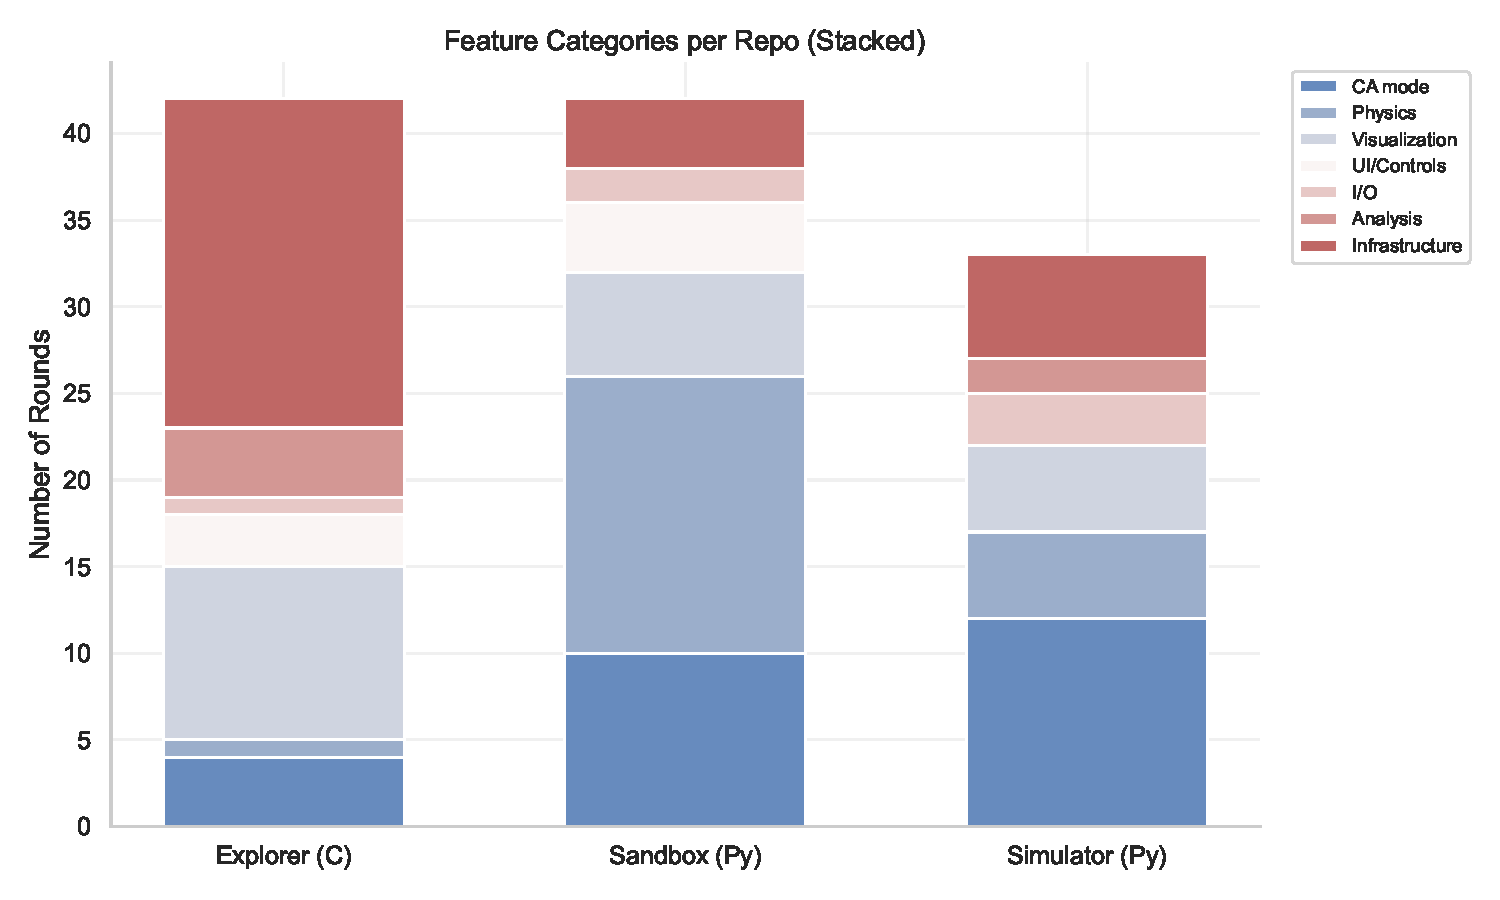
\includegraphics[width=\textwidth]{figures/ralph_feature_categories.pdf}
\caption{Feature categories per repository, classified by keyword matching on each round's Thinker goal. Despite convergent initial goals, the three codebases diverged along orthogonal axes: Explorer toward infrastructure and visualization overlays, Sandbox toward physics simulations and CA rule variants, Simulator toward CA modes and I/O capabilities.}
\label{fig:ralph_features}
\end{figure*}

\textbf{Observation 5: Divergent specialization along orthogonal axes.} Despite identical starting conditions and convergent initial goals, the three codebases specialized in qualitatively different directions (Figure~\ref{fig:ralph_features}). Explorer, written in C, developed deep scientific analysis capabilities: 15+ information-theoretic overlays (Shannon entropy, Lyapunov exponents, transfer entropy, Wolfram classification), multi-rule zones, wormhole portals, and exotic topologies (torus, Klein bottle, M\"obius strip). Sandbox pursued breadth, accumulating 27 interactive simulation modes spanning five categories (cellular automata, physics, biology, procedural generation, algorithms). Simulator combined algorithmic diversity with tooling: 28+ simulation modes alongside genetic algorithm rule discovery, headless batch rendering, and GIF/PNG export.

\begin{figure*}[t]
\centering
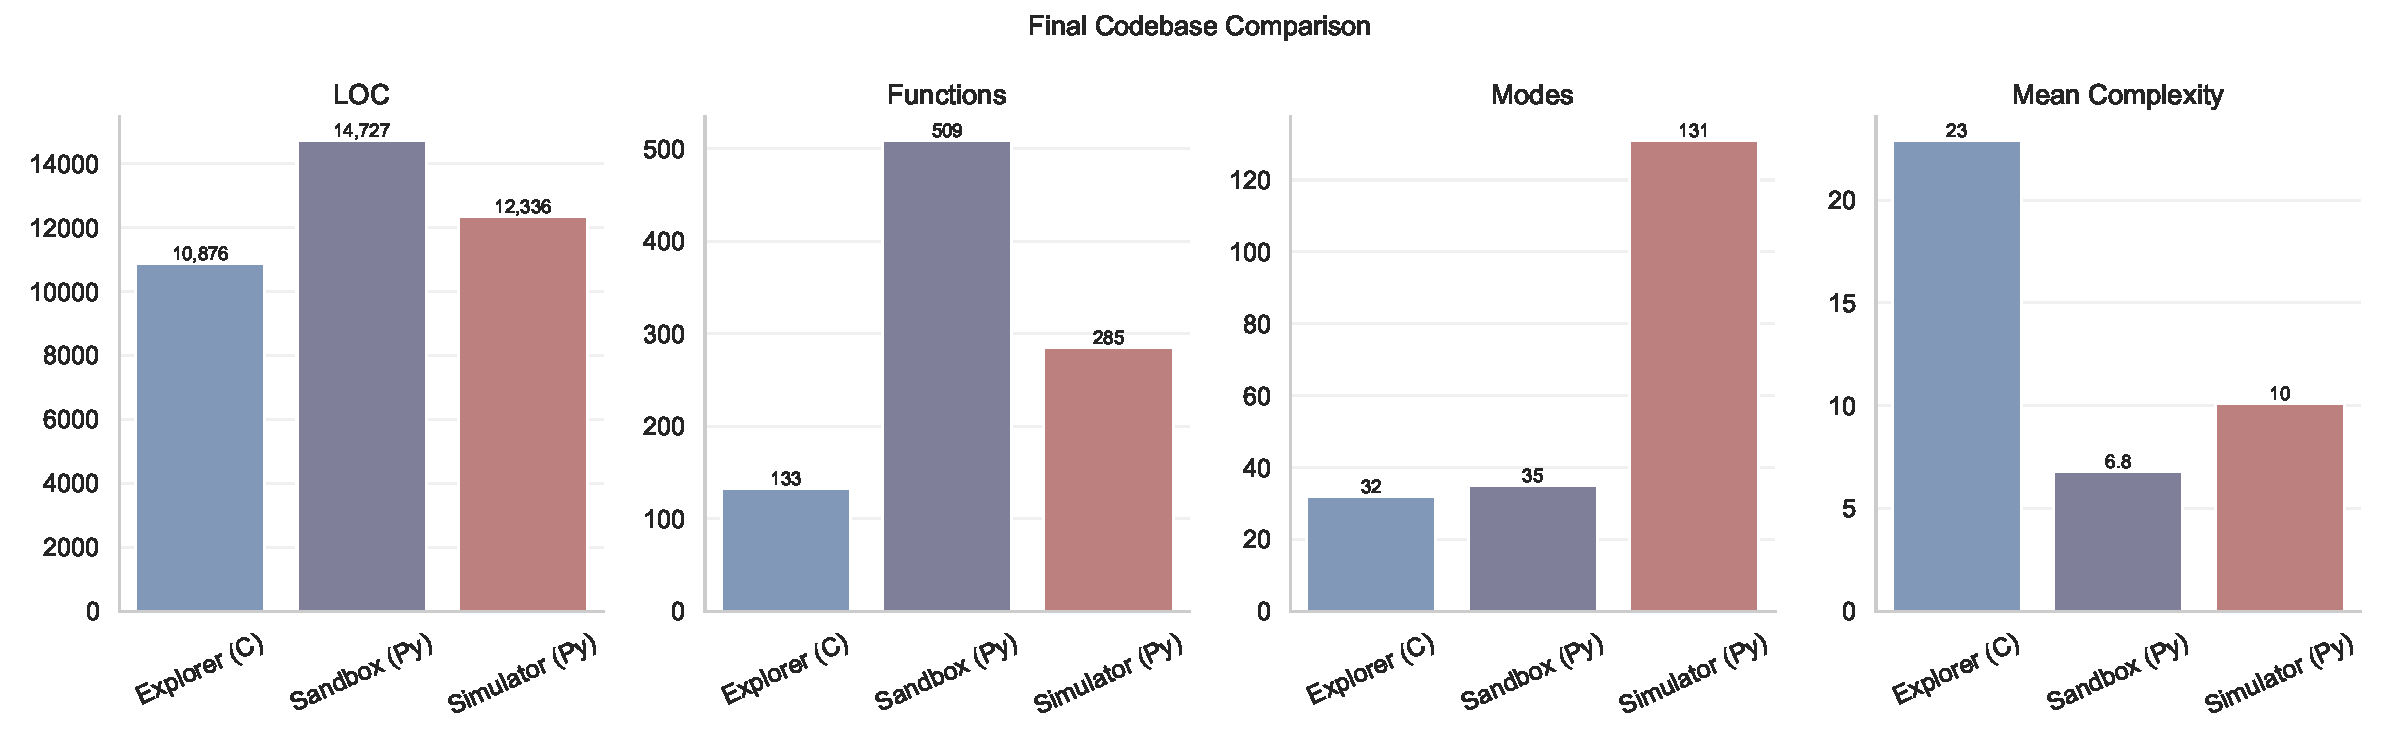
\includegraphics[width=\textwidth]{figures/ralph_final_metrics.pdf}
\caption{Final codebase comparison across four metrics. The Explorer's high mean cyclomatic complexity (22.9 vs.\ 6.8 and 10.1) reflects its C implementation and deeply nested analysis routines. The Simulator's mode count (131) dwarfs the others, reflecting its strategy of adding many small simulation variants.}
\label{fig:ralph_metrics}
\end{figure*}

Figure~\ref{fig:ralph_metrics} quantifies this divergence. The Explorer's mean cyclomatic complexity (22.9) is over three times that of the Sandbox (6.8), reflecting both the inherent verbosity of C and the depth of its analysis routines. The Simulator accumulated the most simulation modes (131) despite having the fewest rounds (33), suggesting a strategy of adding many small, self-contained variants rather than deepening existing ones. This pattern of convergence-then-divergence is consistent with adaptive radiation in evolutionary biology \cite{schluter2000}: a population that enters a new ecological zone (here, the ``cellular automaton niche'') initially exploits the same resources before diverging into specialized sub-niches.

\textbf{Observation 6: Monotonic growth without self-initiated refactoring.} Figure~\ref{fig:ralph_loc} shows that all three codebases grew monotonically, with deletion ratios below 4\%. None of the three instances ever proposed refactoring its own codebase, in contrast with the Wallfacer experiment's Observation~2, where the three-agent configuration proposed refactoring at approximately 51{,}000 lines. We interpret this as negative evidence supporting the fission principle: ralph's fixed thinker-worker-committer loop lacks a Cartographer role that would produce the structured self-representation needed for architectural self-awareness. Without a legible abstraction of global system state, the Thinker's planning horizon remains local --- it can propose the next feature but cannot diagnose structural debt. This suggests that self-diagnostic capability is an emergent property of role differentiation, not an intrinsic capability of the underlying LLM.
